\section{The \resource{} Resource}
\label{sec:rel-graph}

We now create \resource{}, a concrete resource according to the framework described in Section \ref{sec:framework}.
% To measure PLMs' consistency, we test their predictions sensitivity to various paraphrased queries. 
% We create a paraphrase resource that enables us to study this property, which we name \resource{}. \am{last 2 sentences are redundant. keep only the first imo} \resource{} is a high-quality resource, built by experts. %, and results in a high-quality resource which we hope can contribute to others' work as well.
\resource{} is a high-quality resource, built by experts,
it contains patterns for 40 relations from the T-REx dataset \cite{trex}, with an average of @@ patterns per relation.
Some statistics of the resource are presented in Table \ref{tab:rel-graph-stats}.

% Each pattern is represented as a node in an undirected graph, and each edge signifies the type of modification from one pattern to another (e.g. lexical change).
% A schematic view of the ``aired on'' relation can be seen in Figure \ref{fig:graph}. 

% All patterns from a specific relation are paraphrases.
% Each pattern entails the main expression for each pattern, but not necessarily the other way around. 
% For example, for the relation of ``aired on'', which describes a TV-series that was aired on some network, the original pattern is: ``\subj{} was aired on \obj{}'' and one of the patterns we create is ``\subj{} was premiered on \obj{}'', which entails the main expression, but not vice versa.


% For instance, the phrase "\subj{} was aired on \obj{}" entails "\obj{} released \subj{}", but not "\subj{} was premiered on \obj{}", although the other direction is entailed.
% \ar{The entailment 'Y released X' doesn't seem correct. Suggestion For instance, the phrase "\subj{} was premiered on \obj{}" entails "\subj{} was aired on \obj{}", but not the other way around.}

% \begin{figure}[t!]
% \centering

% 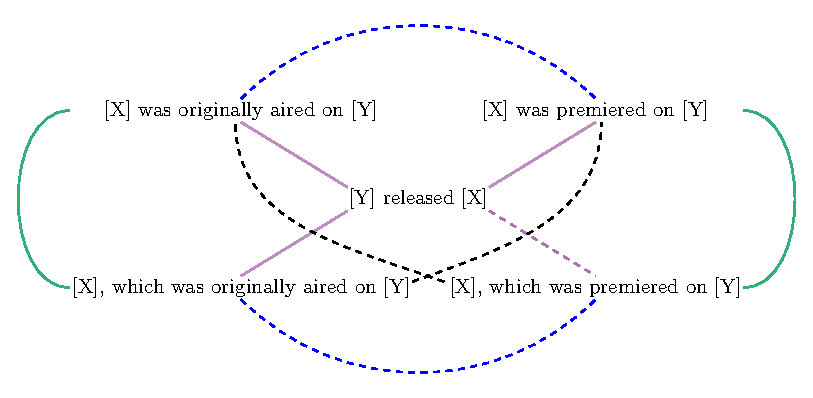
\includegraphics[width=1.\columnwidth]{figures/ent_graph}

% \caption{Overview of \resource{}.}
% \label{fig:graph}
% % \vspace{-6mm}
% \end{figure}

% Overall, \resource{} contains @@ different patterns in total for @@ different relations (@@\% paraphrases per relation in average). 
% All of the paraphrases for a particular relation are organized as a directed graph to indicate the entailment relation between two patterns. 
% Each edge also contains information about the transformation type, e.g. a lexical or syntactic transformation (Examples for each can be seen in Figure \ref{fig:graph}).
%A detailed definition is provided shortly.
% \ye{need to define this.} 
% This information allows us to study the different generalization capabilities of models.
% The nodes of the graph (which account for the phrases), also contain additional information about the number of times that the pattern appeared in Wikipedia, @@ more?. %\ar{will we still have the wikipedia info in the paper?}

\paragraph{Construction Method}
\resource{}, was constructed in four steps: (1) We began with the patterns provided by LAMA \cite{lama} (one pattern per relation, referred to as ``base pattern"); (2) we augmented these patterns with other patterns that are paraphrases of the base pattern. Some of these relations are
taken from LPAQA \cite{alpaqa}. However, since these patterns were extracted automatically, many do not accurately depict the relation, therefore only a subset of these patterns were used in practice;  (3) using SPIKE \cite{spike},\footnote{\url{https://spike.apps.allenai.org/}} a search engine over wikipedia sentencecs that allows syntax-based queries, we searched for additional patterns that appeared in Wikipedia and added them to our resource. This was done by searching for subject and object tuples from the T-REx resource and
looking at the sentences that contain both, followed by a human annotator extracting a pattern from the Wikipedia sentence. (4) Lastly, we added additional patterns that are paraphrases of the base pattern using the annotators' linguistic expertise.
% (The annotators can also add entailing or entailed patterns, but we do not make use of them in this paper.)
Two additional experts went over all the patterns and corrected them, while engaging in a discussion until reaching an agreement, discarding patterns with disagreements.

% \nk{should we give a number?}.\ye{I don't think it's necessary}

% \nk{Not sure if the details of this need to be in the main paper or can be moved to the appendix?} \sr{I support moving the technicalities to an appendix and focus here on the properties of the resources and how it is being used.}
% \ye{can decide when we have the full story}
%The entailment edges were also annotated by the same two authors that created the patterns.

\begin{table}[t]
% \small
    \centering
\begin{tabular}{lr}
\toprule
           stat &   values \\
\midrule
      n. graphs &    15 \\
   avg patterns &    19.73 \\
   min patterns &     9 \\
   max patterns &    37 \\
       n. edges &  4821 \\
 edge syntactic &     0.03 \\
   edge lexical &     0.87 \\
      edge both &     0.09 \\
\bottomrule
\end{tabular}
    \caption{Statistics for \resource{}. \ye{numbers are not updates with all the graphs}}
    \label{tab:rel-graph-stats}
\end{table}


% \paragraph{Consistency Types}
% % \nk{we should change inference types to consistency types} \ye{but the graph is in entailment graph}
% To study the consistency against syntactic and lexical variations of models, each edge is augmented with the type of changes performed to reach from one pattern to another. We account for three types of changes: (1) \textit{syntactic}, (2) \textit{lexical} and (3) \textit{determiner}, all binary variables that account for a change of the specific type between two patterns.
% \textit{Syntactic} structure is defined as the dependency path between the subject and the object in a given pattern, where the path includes the edge types. Two patterns are considered equal syntactically if the labeled paths are identical.
% \textit{Lexical} difference is defined by words difference between two patterns, excluding determiners, punctuation, and symbols. The addition or removal of a preposition does not count as a lexical change.
% \textit{Determiner} difference is considered when the patterns' determiners do not fully overlap.



% and full statistics per relation are presented in Table \ref{tab:rel-graph-stats-elaborate} in the Appendix.


\paragraph{Human Agreement}
To assure the quality of \resource{}, we run a study to test for agreement with our annotations.
For each relation, we sample up to five paraphrases, comparing each of the new patterns to the base pattern that came with that resource, and which is assumed to correctly describe the relation.
By definition, two different patterns that are paraphrases of of the LAMA pattern, are also paraphrases of each other.

We populate the patterns with random subjects and objects from T-REx \cite{trex} and ask annotators if these sentences are paraphrases.
We also sample patterns from different relations to provide examples that are not paraphrases of each other, for control.
Overall, each task contains five patterns that are thought to be paraphrases, and two that are not.\footnote{Note that the control patterns contain the same subject and object for avoiding shortcuts in solving the task.}

We asked graduate students in NLP to perform the annotations and collected one answer per question.
Due to random errors in the annotations, for every question that does not match our original label (either for paraphrases or controls), we ask the annotators to relabel them (without specifying the reason), to allow them to fix random mistakes.\footnote{Moreover, due to the sampling of patterns from different relations, seldom the patterns may be paraphrases of one another, which we do not count as mistakes.}
% \nk{I would cut that last sentence}

The agreement score for the paraphrases and the control are: @@ and @@, which are high and reassures \resource's quality.
We further went through the disagreements  %of the paraphrases 
and fixed any additional problem %that we agree with, 
to further improve the resource quality.
Examples of paraphrases are displayed in Table \ref{tab:predictions}. \am{a bit odd to send the reader all the way to table 4, at this stage}
% \begin{table*}[t]
% \small
    \centering
\resizebox{1\textwidth}{!}{%
\begin{tabular}{llll}
\toprule
           Pattern & Base &  Entailed & Type \\
\midrule
% hi & byw & chao \\
      \textsc{Died-in} & \textsc{Subj} passed away in \textsc{Obj}. & $\Leftrightarrow$ \textsc{Subj} died in OBJ. & lexical \\
       & \textsc{Subj} was murdered at \textsc{Obj}. & $\Rightarrow$ \textsc{Subj} died in \textsc{Obj}. & lexical \& syntactic \\
       & \textsc{Subj} died at \textsc{Obj}. & $\Leftrightarrow$ \textsc{Subj} died in \textsc{Obj}. & lexical \\
       
       \midrule
       
       \textsc{Official-language} & \textsc{Obj} is the official language of \textsc{Subj}. & $\Leftrightarrow$ The official language of \textsc{Subj} is \textsc{Obj}. & syntactic \\
       & In \textsc{Subj} \textsc{Obj} is an official language. & $\Leftrightarrow$ The official language of \textsc{Subj} is \textsc{Obj}.	& \\
       
       \midrule
       
       \textsc{Located-in} & \textsc{Subj} is a county in \textsc{Obj}. & $\Rightarrow$ \textsc{Subj} is located in \textsc{Obj} . & lexical \& syntactic \\
       & \textsc{Subj} district, \textsc{Obj}.	& $\Rightarrow$ \textsc{Subj} is located in \textsc{Obj} . & lexical \& syntactic \\
       
       \midrule
       
       \textsc{Instrument} & \textsc{Subj} was a \textsc{Obj} player. & $\Rightarrow$ \textsc{Subj} plays \textsc{Obj}. & lexical \& syntactic \\
       & \textsc{Subj} played \textsc{Obj} . & $\Leftarrow$ \textsc{Subj} plays \textsc{Obj}. & tense \\
       & \textsc{Obj} sonatas of \textsc{Subj}. & $\Rightarrow$ \textsc{Subj} plays \textsc{Obj}. & lexical \& syntactic \\
       
\bottomrule
\end{tabular}
}
    \caption{Examples of patterns in the \resource{}.}
    \label{tab:rel-graph-examples}
\end{table*}

